\documentclass[12pt]{article}
\usepackage[french]{babel}
\usepackage{natbib}
\usepackage{url}
\usepackage[utf8x]{inputenc}
\usepackage{amsmath}
\usepackage{graphicx}
\usepackage[svgnames]{xcolor}
\usepackage{vmargin}
\setmarginsrb{3 cm}{1 cm}{3 cm}{1.5 cm}{1 cm}{0.5 cm}{1 cm}{1.5 cm}
\usepackage{multirow}
\graphicspath{{images/}}
\usepackage{parskip}
\usepackage{fancyhdr}
\usepackage[T1]{fontenc}
\usepackage{url}
\usepackage{pdfpages}
\usepackage{url}
\usepackage{hyperref}
\usepackage{graphicx}
\usepackage{subfigure}
\usepackage{caption}
\usepackage{subcaption}
\usepackage{empheq, cases}
\usepackage{amssymb}
\usepackage{amsmath}
\usepackage{verbatimbox}
\usepackage{tcolorbox}
\usepackage{float}
\usepackage{multicol}
\usepackage[compact]{titlesec}
\usepackage[colorinlistoftodos]{todonotes}
\usepackage{sectsty}
\titlespacing{#1}{1}{#3}





\xdefinecolor{gray}{named}{lightgray}
\xdefinecolor{alice}{named}{AliceBlue}
\xdefinecolor{saumon}{named}{PeachPuff}
\definecolor{myred1}{RGB}{255, 0, 0}
\definecolor{mygreen1}{RGB}{0, 126, 0}
\definecolor{myblue1}{RGB}{0, 0, 61}
\definecolor{lightgray}{rgb}{0.83, 0.83, 0.83}
\definecolor{brick}{rgb}{0, 0, 0.50}
\sectionfont{\color{brick}}  % sets colour of chapters
\subsectionfont{\color{RoyalBlue}}

\tcbset{colback=lightgray,colframe=black}



\title{\color{brick} Optimisation TD 4:\\
\LARGE{Recuit simulé et le voyageur de commerce}}								% Title
\author{Émilie Mathian}								% Author
\date{Année 2018 - 2019}											% Date

\makeatletter
\let\thetitle\@title
\let\theauthor\@author
\let\thedate\@date
\makeatother

\pagestyle{fancy}
\fancyhf{}
\rhead{\theauthor}
\lhead{Optimisation TD 1}
\cfoot{\thepage}
%%%%%%%%%%%%%%%%%%%%%%%%%%%%%%%%%%%%%%%%%%%%%%%%%%%%%%%%%%%%%%%
\usepackage{eso-pic}
\newcommand\BackgroundPic{%
\put(0,0){%
\parbox[b][\paperheight]{\paperwidth}{%
\vfill
\centering
\includegraphics[width=\paperwidth,height=\paperheight,%
keepaspectratio]{background.png}%
\vfill
}}}
  
  
\begin{document}

%%%%%%%%%%%%%%%%%%%%%%%%%%%%%%%%%%%%%%%%%%%%%%%%%%%%%%%%%%%%%%%%%%%%%%%%%%%%%%%%%%%%%%%%%

\begin{titlepage}
	\centering
    \vspace*{0.5 cm}
    \vspace{-3.5cm}
    
\includegraphics[width = 4cm]{logo.png}\\	% University Logo
    \textsc{\LARGE Institut National des Sciences Appliquées de Lyon}\\[2.0 cm]	% University Name
	\textsc{\Large $4^{eme}$ Année Bioinformatique et Modélisation}\\[0.5 cm]				% Course Code
	\textsc{\large Professeur: Noëlie DEBS }\\[0.5 cm]				% Course Name
	\rule{\linewidth}{0.2 mm} \\[0.4 cm]
	{ \huge \bfseries \thetitle}\\
	\rule{\linewidth}{0.2 mm} \\[1.5 cm]
	
	\begin{minipage}{0.4\textwidth}
		\begin{flushleft} \large
			\emph{Auteur:}
			\theauthor
			\end{flushleft}
			\end{minipage}~
			\begin{minipage}{0.4\textwidth}	
	\end{minipage}\\[2 cm]
    \vspace{-1.8cm}
	 \begin{figure}[H]
	\begin{center}
	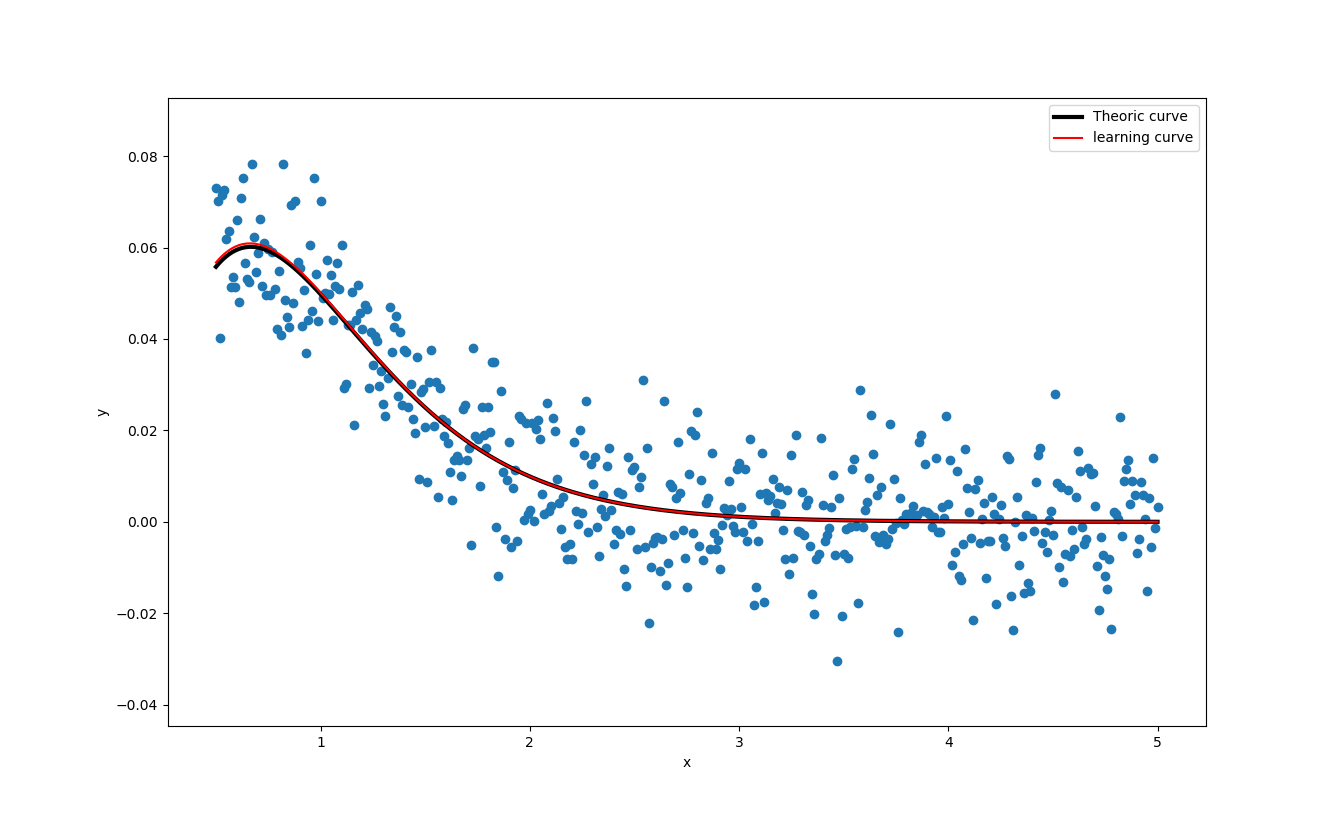
\includegraphics[width=0.9 \textwidth]{Figure_1.png}
\end{center}
\end{figure}

	{\large \thedate}\\[1 cm]
    
	\vfill

 

\end{titlepage}
\pagebreak
%%%%%%%%%%%%%%%%%%%%%%%%%%%%%%%%%%%%%%%%%%%%%%%%%%%%%%%%%%%%%%%%%%%%%%%%%%%%%%%%%%



\newpage 

\tableofcontents

\newpage

\section{Le recuit simulé}
\begin{center}
\fcolorbox{black}{lightgray}{
\begin{minipage}{\linewidth}
\textbf{Problématique :} \\
Le recuit simulé est un algorithme d'optimisation intégrant une part d'aléatoire. Cet algorithme est une analogie à une technique employée en métallurgie, où la fonction à minimiser est l'énergie libre d'un système. On voudrait ainsi obtenir un métal ayant la plus grande stabilité soit un cristal, or cet état n'est atteint que lorsque le processus de refroidissement est lents, sinon on risque d'obtenir un polycristal de plus haute énergie libre. Nous étudierons  ainsi l'effet du 'refroidissement'. De plus par analogie à la thermodynamique, si l'on considère un système à l'équilibre à une température T, ce système a une probabilité faible de changer d'état et cette probabilité décroît avec T (probabilité de Boltzmann). Nous observerons l'importance de cette loi qui donne de la souplesse à l'algorithme.\\
Le rapport suivant reprend le programme \textit{'recuit.py'}.
\end{minipage}}
\end{center}


\subsection{Fonction de $\mathbb{R}$ dans $\mathbb{R}$}
\begin{minipage}{0.5\textwidth}

\textbf{\color{brick}1.} 
D'après la représentation de la fonction $f(x)$ \textbf{[\ref{Q1}}, nous observons l'existence d'un minimum local et d'un global, et d'un maximum local. Nous pouvons numéiquement estimer les coordonnées de ces points d'inflexion. Le minimum local est atteint pour $x\simeq 2.823$ alors $f(2.823)\simeq -114.55$, le maximum local est atteint pour $x\simeq0.024$ alors $f(0.024)\simeq 1.012$ et enfin le minimum global est atteitn pout $x\simeq 3.548$ et alors $f(3.548)\simeq -133.41$.
\end{minipage} \hfill
\begin{minipage}{0.45\textwidth}
\begin{figure}[H]
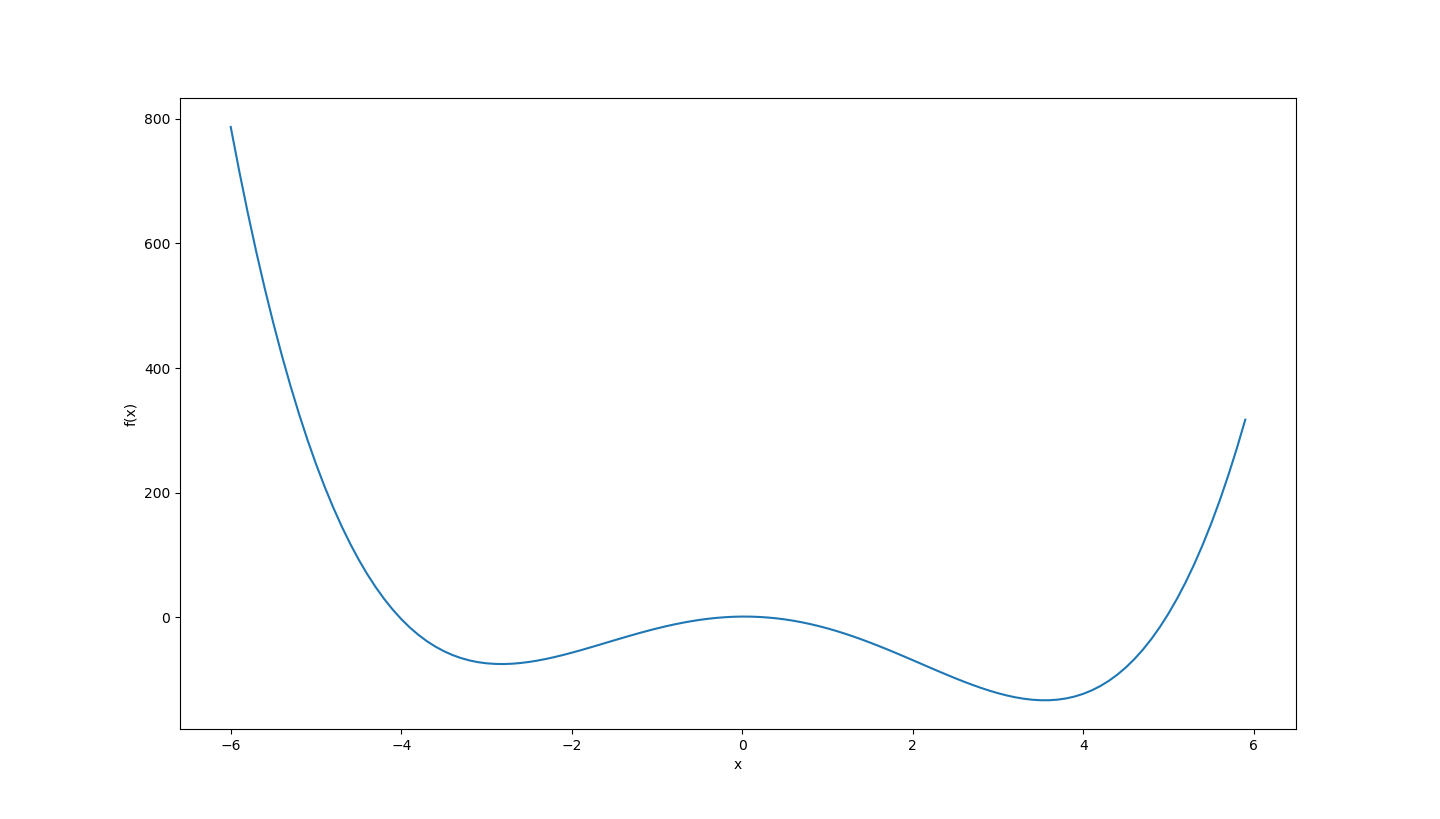
\includegraphics[width=1\textwidth]{Q1.png}
\caption{Représentation de la fonction à minimiser  $f(x)=x^4 - x^3 -20x^2+x+1$}
\label{Q1}
\end{figure}
\end{minipage}


\begin{minipage}{0.5\textwidth}
\textbf{\color{brick}2.} L'implémentation de la méthode du recuit simulé pour la fonction $f$ décrite ci-dessus fait référence à la fonction \verb|recuit_f1| (cf : \verb|recuit.py|).\\
 Pour tester notre algorithme nous prenons les conditions suivantes : $k=10$, $k'=0.5$, $T=1/t$ et $t_{max}=1$, la solution obtenue est illustrée ci-contre \textbf{[\ref{Q1_2}]}. Nous remarquons que la solution converge vers le minimum global, avec comme résultat final $x_{t=10000} \simeq 3.548  $ et $f(x_{t=10000}) \simeq -133.41$. En revanche l'algorithme a parcouru un vaste espace et des valeurs très éloignées de la solution avant de cnverger.
\end{minipage} \hfill
\begin{minipage}{0.45\textwidth}
\begin{figure}[H]
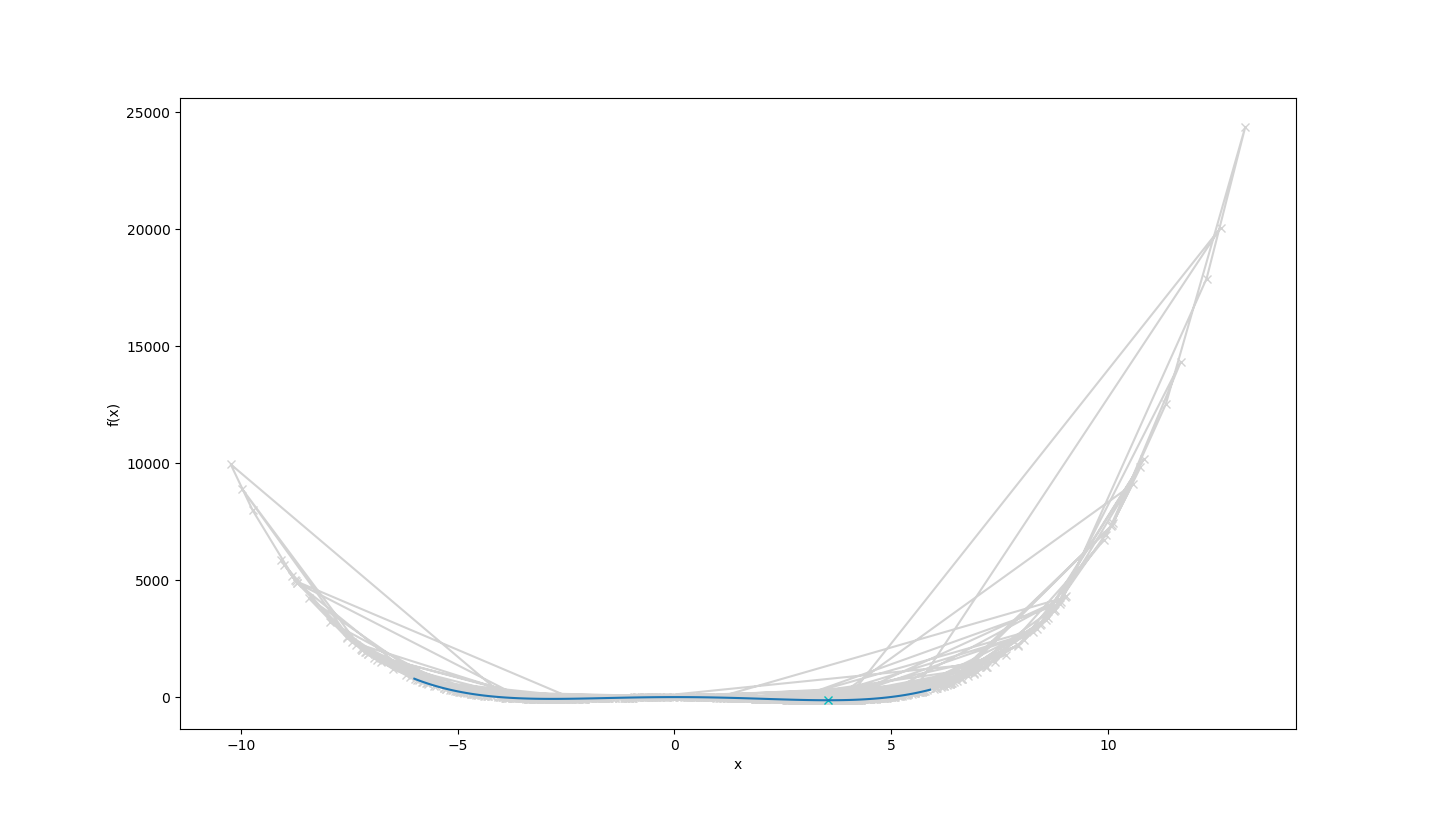
\includegraphics[width=1\textwidth]{Q1_2.png}
\caption{Représentation de la fonction à minimiser  $f$, du parcours de l'algorithme du recuit simulé et de la solution finale retenue.}
\label{Q1_2}
\end{figure}
\end{minipage}

\begin{figure}[H]
  \centering
  \subfigure[Variation de k]{%
    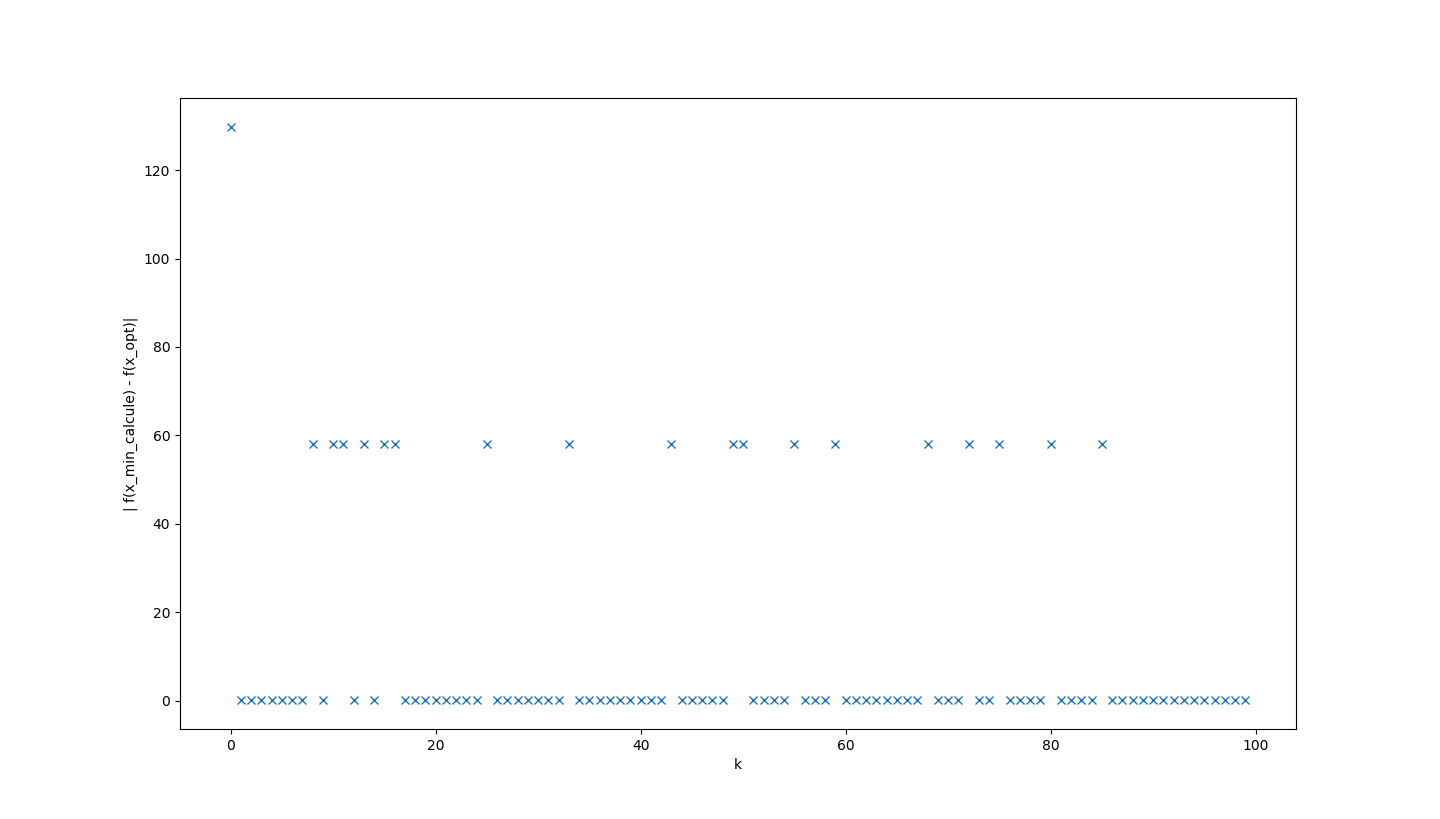
\includegraphics[width=0.45\textwidth]{Q1_k.png}
    \label{fig:a}%
    }%or more
    \subfigure[Variation de k']{%
    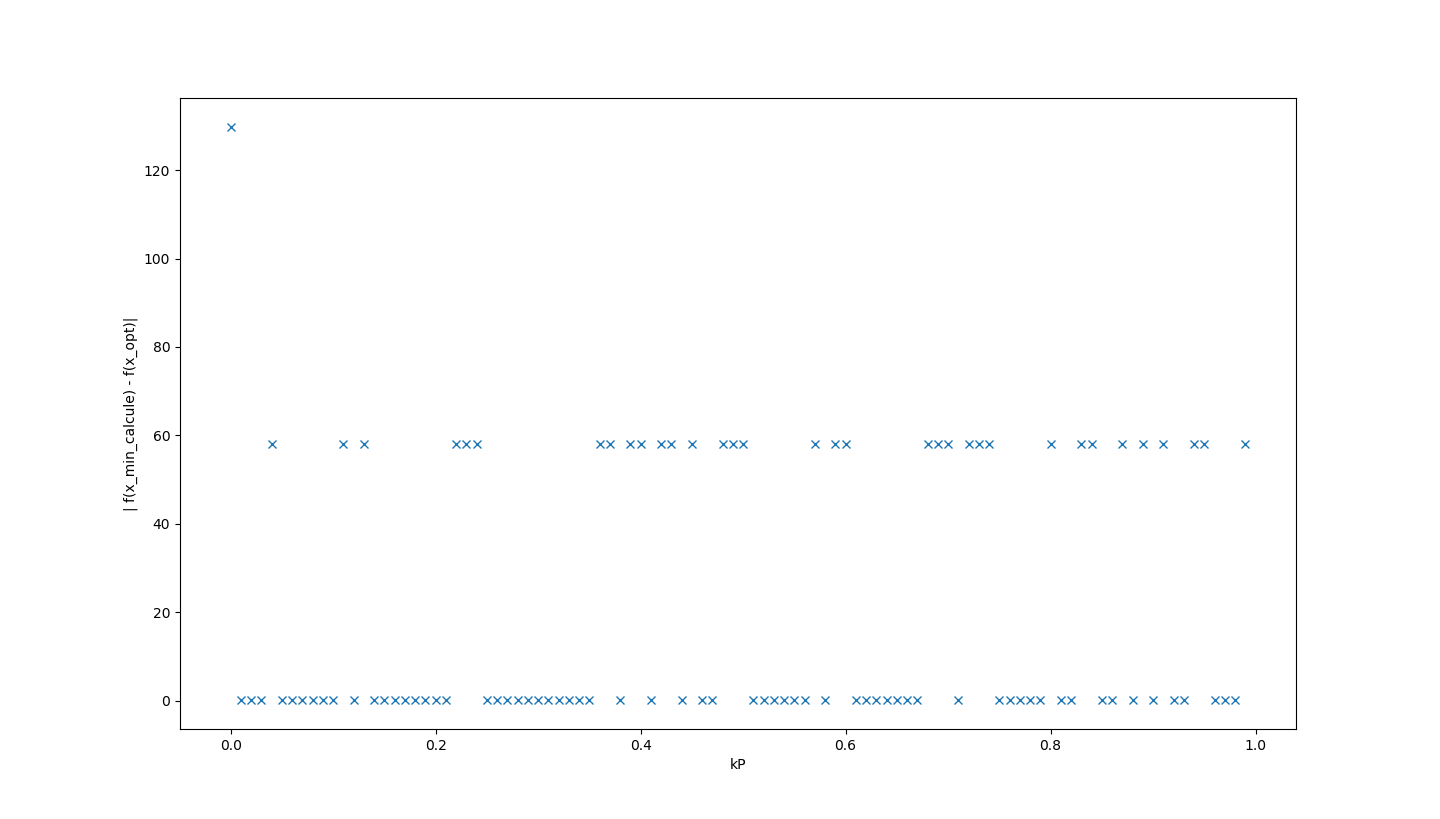
\includegraphics[width=0.45\textwidth]{Q1_kp.png}
    \label{fig:b}%
  }%  
  \caption{Étude de l'écart entre la solution calculée et la solution analytique pour 10000 itération avec $x_0 = 0.5$, et pour \textbf{a} $kp=0.5$ et $k\in [0,30]$ et  pour \textbf{b} $kp \in [0,1]$ et $k= 10$}
  \label{fig:ab}
\end{figure}
D'après la figure \textbf{[\ref{fig:a}]}, on observe que l'algorithme converge plus fréquemment vers le minimum local lorsque k est faible, la densité du nuage de point, pour $f(\hat{x_opt}- f(x_opt)) \simeq 60$ , est plus forte à gauche. Ainsi plus on permet à l'algorithme d'inspecter un voisinage éloigné du $x$ courant plus  la probabilité de trouver le minimum global croit.  À l'inverse d'après la figure \textbf{[\ref{fig:b}]} plus $k'$ augmente (noté kp) augmente plus la probabilité de converger vers le minimum local augmente, la densité du nuage de point pour  $f(\hat{x_opt}- f(x_opt)) \simeq 60$ , est plus forte à droite. Ainsi plus on abaisse la probabilité d'accepter un point qui augmentait localement le coût plus la probabilité de converger vers le minimum global croît.

\begin{minipage}{0.5\textwidth}

D'après la figure \textbf{[\ref{Q1_T}]}, nous observons que si le nombre d'itération est trop faible $t_{max}<1500$ l'algorithme n'a pa le 'temps' de converger si $t_{max}$ est supérieur à ce seuil alors l'algorithme convergera vers l'un des deux minimums.
\end{minipage} \hfill
\begin{minipage}{0.45\textwidth}
\begin{figure}[H]
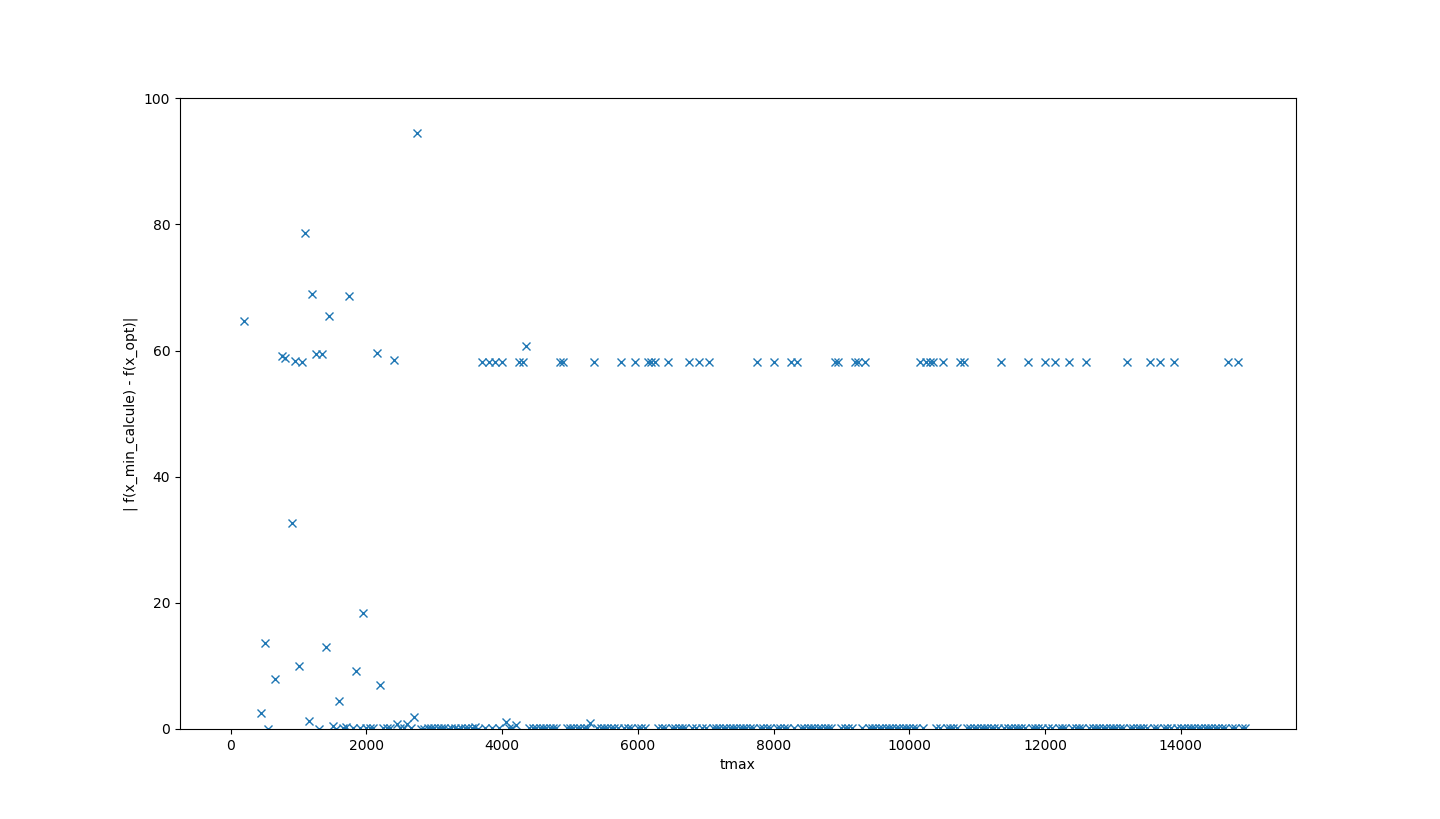
\includegraphics[width=1\textwidth]{Q1_T.png}
\caption{valeur absolue de l'erreur en fonction du nombre d'itération maximal}
\label{Q1_T}
\end{figure}
\end{minipage}



\begin{minipage}{0.5\textwidth}
Rappelons que le choix du nombre d'itérations maximale influence également la température étant donnée que $T=\frac{1}{t}$, pour observer l'influence de la température nous pouvons faire varier le coefficient  '1000' pour ralentir ou augmenter le processus de refroidissement. Nous faisons donc varier ce coefficient entre $[0,2000]$ et nous obtenons les résultats ...
% Ref image
\end{minipage} \hfill
\begin{minipage}{0.45\textwidth}
\begin{figure}[H]
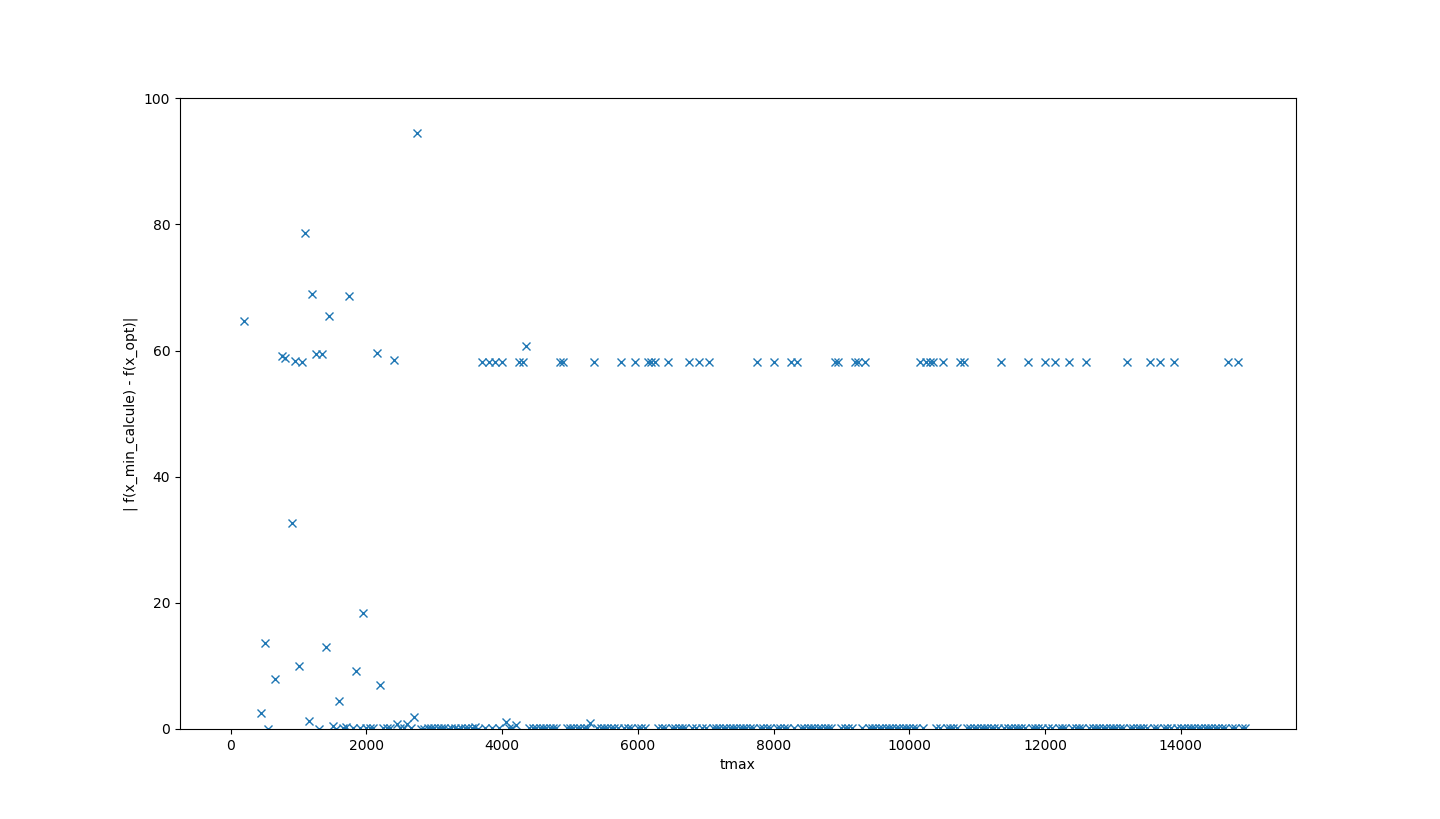
\includegraphics[width=1\textwidth]{Q1_T.png}
\caption{valeur absolue de l'erreur en fonction du nombre d'itération maximal}
\label{Q1_T}
\end{figure}
\end{minipage}

\textbf{\color{brick}3.} D'après les analyses précédentes pour augmenter la convergence de l'algorithme vers le minimum global nous choisissons $k=20$, $k'p=0.1$ et $t_{max}=15000$, nous obtenons alors les résultats suivants:
\begin{figure}[H]
\centering
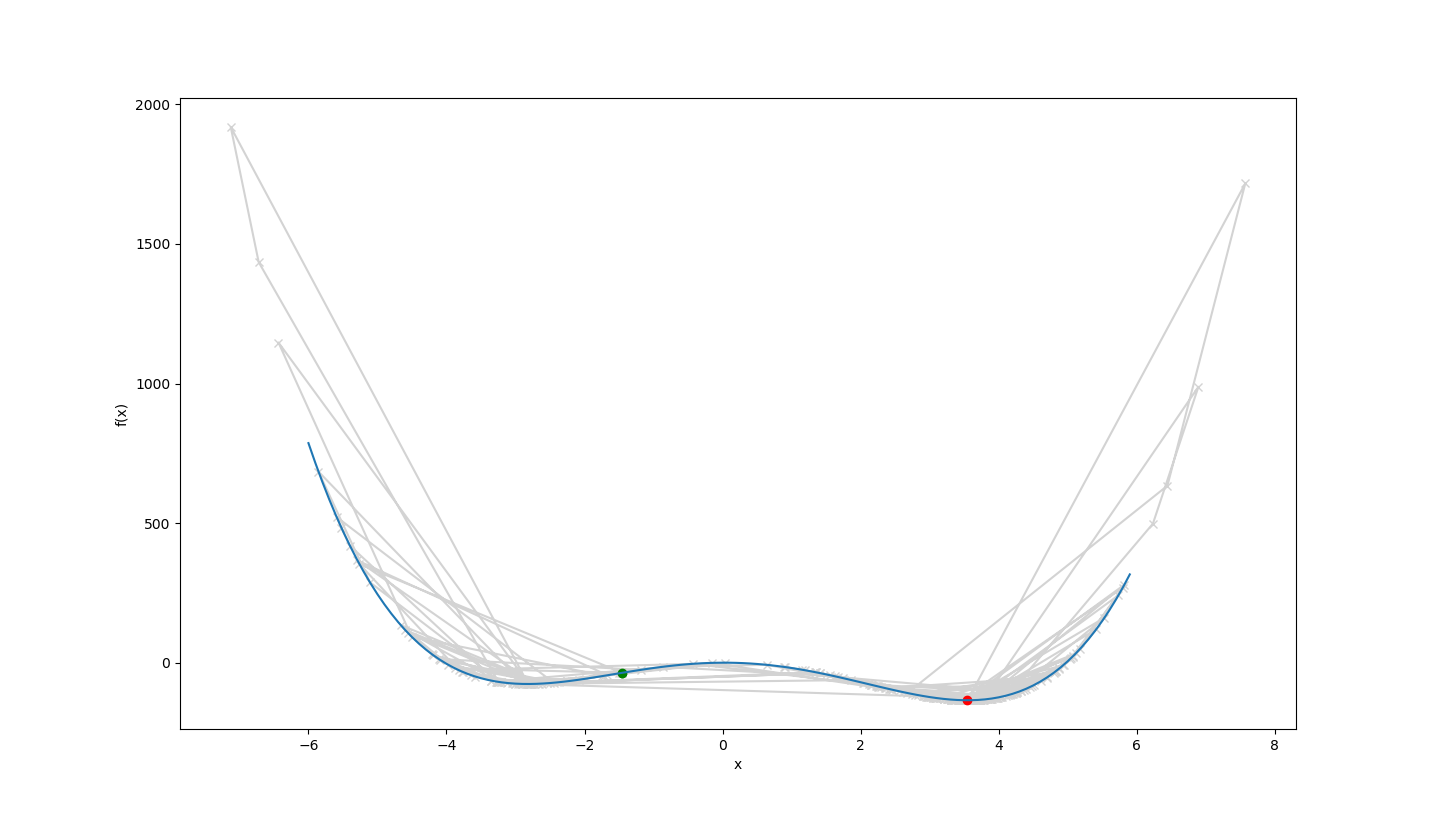
\includegraphics[width=0.8\textwidth]{Q132.png}
\caption{Représentation de l'évolution de l'algorithme (gris), à la surface de $f$ (bleu), le point de départ est indiqué en vert et celui d'arrivée en rouge.}
\label{Q1_T}
\end{figure}

\begin{center}
\fcolorbox{black}{lightgray}{
\begin{minipage}{\linewidth}
\textbf{Remarque sur l'algorithme :} \\
\begin{itemize}
    \item Le point de départ est choisi aléatoirement dans une lois uniforme selon deux bornes données par l'utilisateur.
    \item En plus du critère d'arrêt établi par rapport à un nombre d'itérations, une seconde condition d'arrêt a été établi sur le pourcentage d'acceptation, c'est à dire le nombre de mouvement retenu par rapport au nombre d'itérations total. On peut en effet estimer que si ce pourcentage est faible alors l'algorithme ne conserve que très rarement des solutions, et est donc dans un minimum local de la fonction de coût.\\
    
\end{itemize}
\end{minipage}}
\end{center}
\newpage
\subsection{Fonction de $\mathbb{R^2}$ dans $\mathbb{R}$}
Nous étudions la fonction $g(x,y)= x^4-x^3-20x^2+x+1 +y^4-y^3-20y^2+y+1$; cette fonction a été dans le TD 1 exercice 3; ainsi nous savons qu'elle possède 9 points caractéristique, un maximum local, quatre points selle , et 4 minimum dont un minimm global.

   \end{document}